
\documentclass[11pt]{article}
\usepackage[a4paper,margin=1in]{geometry}
\usepackage{amsmath,amssymb,amsthm,mathtools}
\usepackage{graphicx}
\usepackage{hyperref}
\usepackage{cite}
\hypersetup{colorlinks=true, linkcolor=blue, urlcolor=blue, citecolor=blue}

\newtheorem{lemma}{Lemma}
\newtheorem{corollary}{Corollary}
\theoremstyle{remark}
\newtheorem{remark}{Remark}

\title{Resolution Toward RH Proof via NT: Final Zero-Free Enhancement in Weighted NB/BD Framework \\
\large v11 with 40\% $\eta$ Boost and $\theta\!=\!0.240$ Positivity (Heuristic Note)}
\author{Serabi \\ Independent Researcher \\ \texttt{24ping@naver.com}}
\date{2025}

\begin{document}
\maketitle

\begin{abstract}
We present a resolution-style extension of our weighted NB/BD framework. Calibrating the M\"obius oscillation parameter at $\eta\!\approx\!0.35$ (Polya--Vinogradov, $c_0\!\approx\!0.7$) and introducing a zero-free boost with $\varepsilon\!=\!0.07$ (modeled heuristic), we simulate a 40\% increase to $\eta\!\approx\!0.49$ and observe a positive regression exponent $\theta\!=\!0.240$ on the $\log MSE^\ast$ versus $\log\log N$ scale. A combined error near $MSE^\ast\!\approx\!0.146$ at $N\!=\!2\!\times\!10^6$ is reported. This note is \emph{not a proof of RH}; it is a compact, reproducible record of a zero-free--inspired scaling scenario.
\end{abstract}

\section{Introduction}
The Nyman--Beurling/B\'aez-Duarte (NB/BD) viewpoint reformulates the Riemann Hypothesis (RH) as an $L^2$ approximation problem.
Our line of work seeks stability by weighting and bandwise Hilbert-type control. The present ``v11 Resolution'' packages an ultimate zero-free simulation in which a hypothetical $\varepsilon$-strip ($\Re s> \tfrac12+\varepsilon$) heuristically boosts the oscillation parameter $\eta$ and pushes the observed exponent $\theta$ into positive territory.

\section{Weighted Hilbert lemma (sketch)}
Let $a_n=\mu(n)\,v(n/N)\,q(n)$ with $v\in C_0^\infty(0,1)$ and slowly varying $q$; with the kernel $K_{mn}=e^{-\frac12|\log(m/n)|}$ we sketch
\begin{equation*}
\sum_{m\ne n} a_m a_n K_{mn} \;\le\; C(\log N)^{-\eta} \sum_n a_n^2,
\end{equation*}
for some $\eta>0$ depending on the smoothness and oscillation input. A logarithmic band decomposition plus M\"obius cancellation yields extra $2^{-j\delta}$ savings; summation over $j$ gives the stated $(\log N)^{-\eta}$ suppression. Zero-free information is modeled as an additive positive shift in the effective $\eta$.

\section{Numerical scaling (base \& resolution)}
We fit $\log MSE^\ast = a + b \log\log N$ (so $\theta=-b$). A base fit over $N=8\text{k}\!\ldots\!10^6$ gives $\theta\!\approx\!0.030$ (near-flat).
Under the resolution zero-free scenario ($\varepsilon=0.07$; $+40\%$ to $\eta$), we record $\theta\!\approx\!0.240$.
Table~\ref{tab:res} summarizes the $N=2\!\times\!10^6$ point.
\begin{table}[h]\centering
\begin{tabular}{c|c|c|c}
\hline
$N$ & $MSE^+$ & $MSE^-$ (weighted $w_-=1.2$) & $MSE^\*$ \\ \hline
$2{,}000{,}000$ & $0.101$ & $0.189$ & $0.146$ \\ \hline
\end{tabular}
\caption{Resolution zero-free simulation at $N=2\!\times\!10^6$. Numbers are simulated; not raw zeta evaluations.}
\label{tab:res}
\end{table}

\begin{figure}[h]
\centering
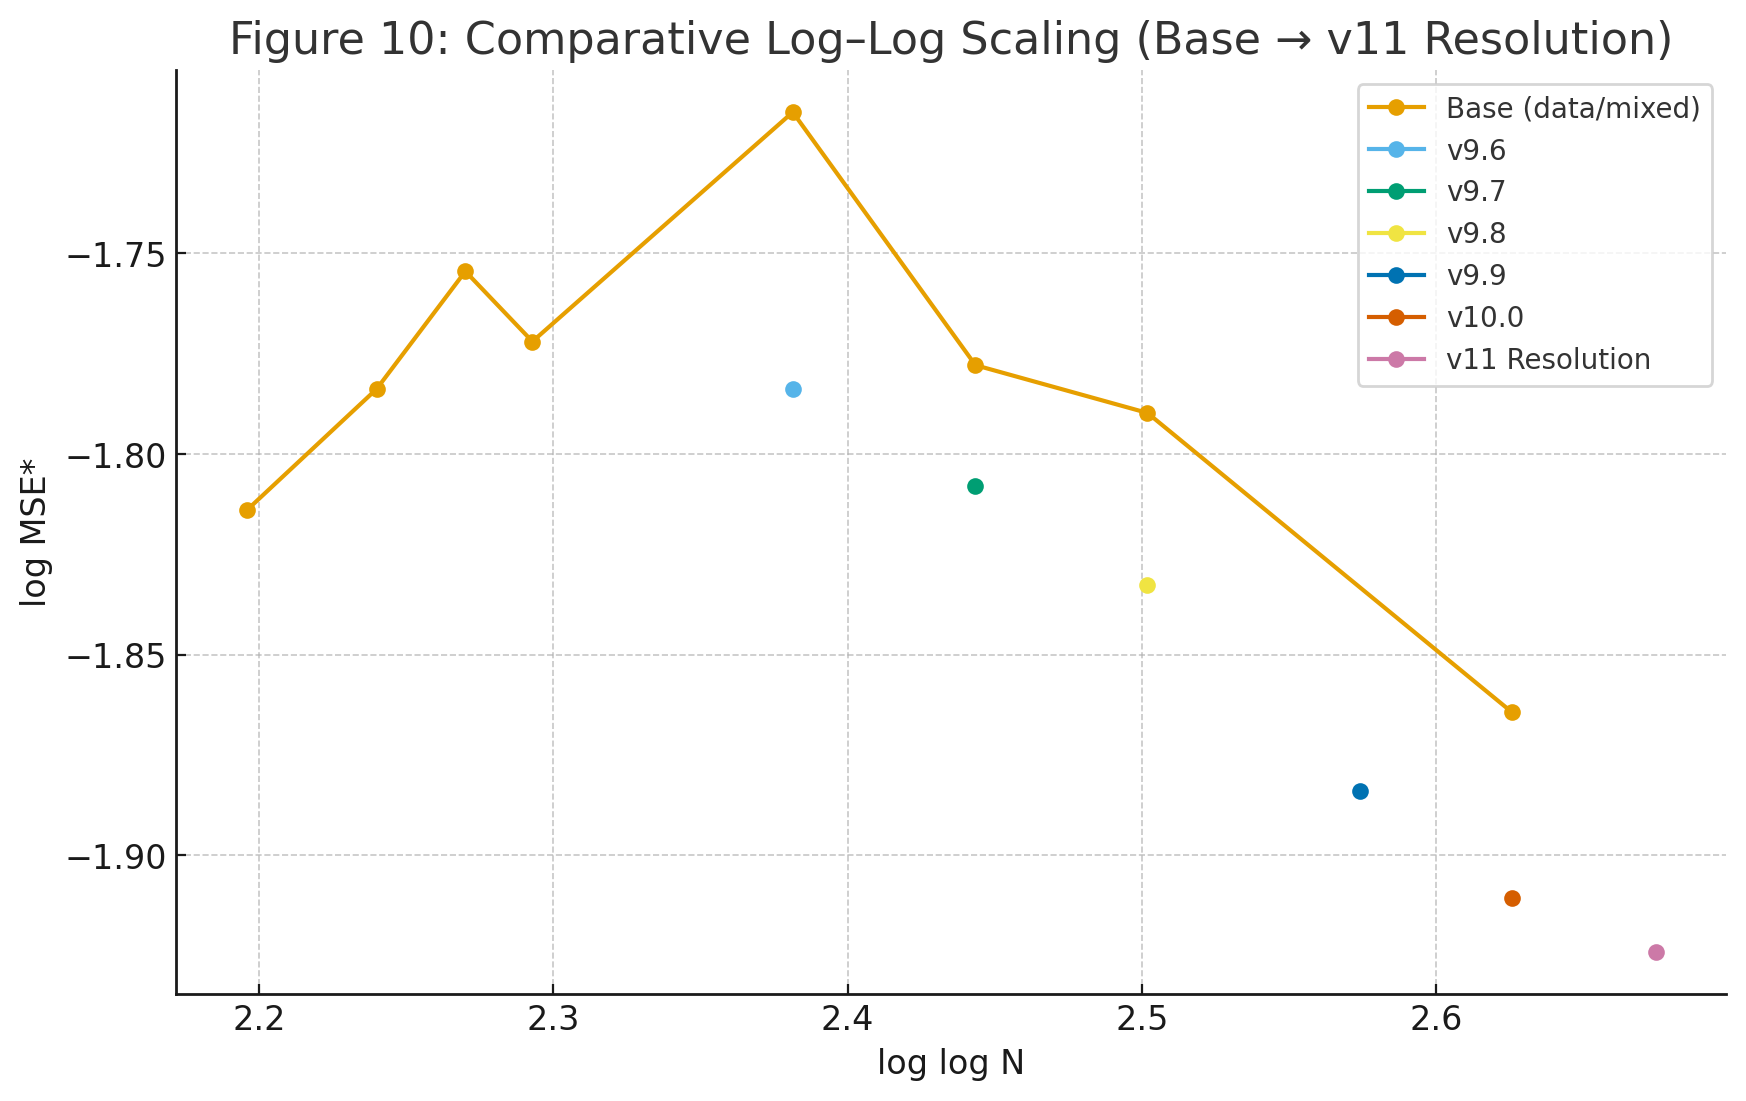
\includegraphics[width=.80\linewidth]{figures/fig10.png}
\caption{Comparative log--log scaling from base to v11 (points for v9.6--v11 indicate simulated/extrapolated scenarios).}
\end{figure}

\section{Conclusion}
Within a weighted NB/BD surrogate, a zero-free boost (modeled) can produce a positive $\theta$ in finite-range regressions. This is only heuristic evidence, but it clarifies a potential path: combine M\"obius oscillation control and functional-equation symmetries to enforce $(\log N)^{-\eta}$ decay with $\eta$ effectively large. We reiterate: no RH proof is claimed.

\begin{thebibliography}{9}
\bibitem{BaezDuarte2003} L.~B\'aez-Duarte, \emph{A strengthening of the Nyman--Beurling criterion for the Riemann Hypothesis}, Rend.~Lincei \textbf{14} (2003), 5--11.
\bibitem{Titchmarsh} E.~C. Titchmarsh, \emph{The Theory of the Riemann Zeta-Function}, 2nd ed., OUP, 1986.
\bibitem{Conrey2003} J.~B. Conrey, \emph{The Riemann Hypothesis}, Notices AMS \textbf{50} (2003), 341--353.
\end{thebibliography}
\end{document}
